\documentclass[conference]{IEEEtran}
\IEEEoverridecommandlockouts
% The preceding line is only needed to identify funding in the first footnote. If that is unneeded, please comment it out.

\usepackage{cite}

\usepackage{amsmath,amssymb,amsfonts}
\usepackage{algorithmic}
\usepackage{graphicx}
\usepackage{textcomp}
\usepackage{xcolor}

% Tables
\usepackage{tabularx}

% Deutsch
\usepackage[ngerman]{babel}
\usepackage[T1]{fontenc}
\usepackage{microtype}

\def\BibTeX{{\rm B\kern-.05em{\sc i\kern-.025em b}\kern-.08em
    T\kern-.1667em\lower.7ex\hbox{E}\kern-.125emX}}
\begin{document}

\title{Autonome KI-Agenten: Technologische Entwicklungen und Anwendungsfelder}

\author{\IEEEauthorblockN{Daniel Vera Gilliard}
\IEEEauthorblockA{\textit{Fakultät Informatik und Wirtschaftsinformatik} \\
\textit{Hochschule Karlsruhe - University of Applied Sciences}\\
Karlsruhe, Deutschland \\
veda1012@h-ka.de}
\and
\IEEEauthorblockN{Robin Gscheidle}
\IEEEauthorblockA{\textit{Fakultät Informatik und Wirtschaftsinformatik} \\
\textit{Hochschule Karlsruhe - University of Applied Sciences}\\
Karlsruhe, Deutschland \\
gsro1011@h-ka.de}}

\maketitle

\begin{abstract}
Autonome KI-Agenten sind eine der fortschrittlichsten Technologien der modernen Informatik, die in der Lage sind, selbstständig Entscheidungen zu treffen und komplexe Aufgaben in verschiedensten Umgebungen zu lösen. Diese Arbeit beleuchtet die technologischen Entwicklungen und Anwendungsfelder autonomer KI-Agenten, mit besonderem Fokus auf Generative Pre-trained Transformer (GPT) und deren Ableitungen wie Auto-GPT und AgentGPT. Weiterhin werden die historischen Meilensteine und technologischen Grundlagen dieser Systeme dargestellt. Eine SWOT-Analyse zeigt sowohl die Potenziale als auch die Herausforderungen und Bedrohungen auf, denen autonome KI-Agenten gegenüberstehen. Zusätzlich werden zukunftsweisende Trends wie Hyperpersonalisierung, multimodale KI-Systeme, die Integration von KI in der Biotechnologie und Explainable AI (XAI) diskutiert. Diese Analyse zielt darauf ab, ein umfassendes Verständnis der aktuellen und zukünftigen Entwicklungen im Bereich autonomer KI-Agenten zu vermitteln und deren Implikationen für verschiedene Branchen aufzuzeigen.
\end{abstract}

\begin{IEEEkeywords}
Autonomous AI Agents, Machine Learning, Generative Pre-trained Transformer (GPT), Auto-GPT, AgentGPT, Virtual Agents, Ethical Considerations, Reinforcement Learning
\end{IEEEkeywords}

\section{Einführung}
\subsection{Bedeutung und Relevanz des Themas}

Autonome KI-Agenten zählen zu den spannendsten und dynamischsten Fortschritten der modernen Technologie. Diese Systeme können eigenständige Entscheidungen treffen, komplexe Aufgaben lösen und in unterschiedlichsten Umgebungen agieren, ohne menschliches Eingreifen zu benötigen. Die Entwicklung autonomer KI-Agenten hat bedeutende Fortschritte in der Robotik, im maschinellen Lernen und in der künstlichen Intelligenz hervorgebracht. Ihre Anwendungsfelder erstrecken sich über zahlreiche Branchen, von der industriellen Automatisierung\cite{evjemo_trends_2020} und der Logistik bis hin zu Gesundheitswesen\cite{liu_application_2021}, Finanzdienstleistungen und dem autonomen Fahren\cite{dikmen_autonomous_2016}. Die Relevanz autonomer KI-Agenten liegt in ihrem Potenzial, Effizienz und Produktivität drastisch zu steigern, menschliche Arbeitskräfte zu entlasten und neue Möglichkeiten für Innovationen zu eröffnen. Trotz der beeindruckenden Fortschritte und der breiten Anwendungsfelder stehen autonome KI-Agenten jedoch vor bedeutenden Herausforderungen, einschließlich der Komplexität der Implementierung, ethischen und sicherheitstechnischen Bedenken sowie der Notwendigkeit für robuste und transparente Entscheidungsprozesse. Dieses Paper zielt darauf ab, ein tiefgehendes Verständnis der aktuellen und zukünftigen Entwicklungen im Bereich autonomer KI-Agenten zu vermitteln. Es beleuchtet die technologischen Fortschritte, insbesondere im Kontext von Generative Pre-trained Transformer (GPT) und deren Ableitungen wie Auto-GPT und AgentGPT. Zudem werden die historischen Meilensteine und technologischen Grundlagen dieser Systeme dargestellt, eine SWOT-Analyse durchgeführt und zukunftsweisende Trends wie Hyperpersonalisierung, multimodale KI-Systeme und Explainable AI (XAI) diskutiert.

\section{Technologische Grundlagen}

Autonome Agenten basieren auf verschiedenen technologischen Entwicklungen aus dem Bereich der Sprachmodelle und des Natural Language Processing (NLP) und nutzen Dialogsysteme, um mit dem Benutzer zu interagieren. Diese Systeme sind das Ergebnis umfangreicher Forschung und Entwicklung in den Bereichen maschinelles Lernen und künstliche Intelligenz.

\subsection{Generative Pre-trained Transformer (GPT)}

\begin{figure*}[!htbp]
    \centering
    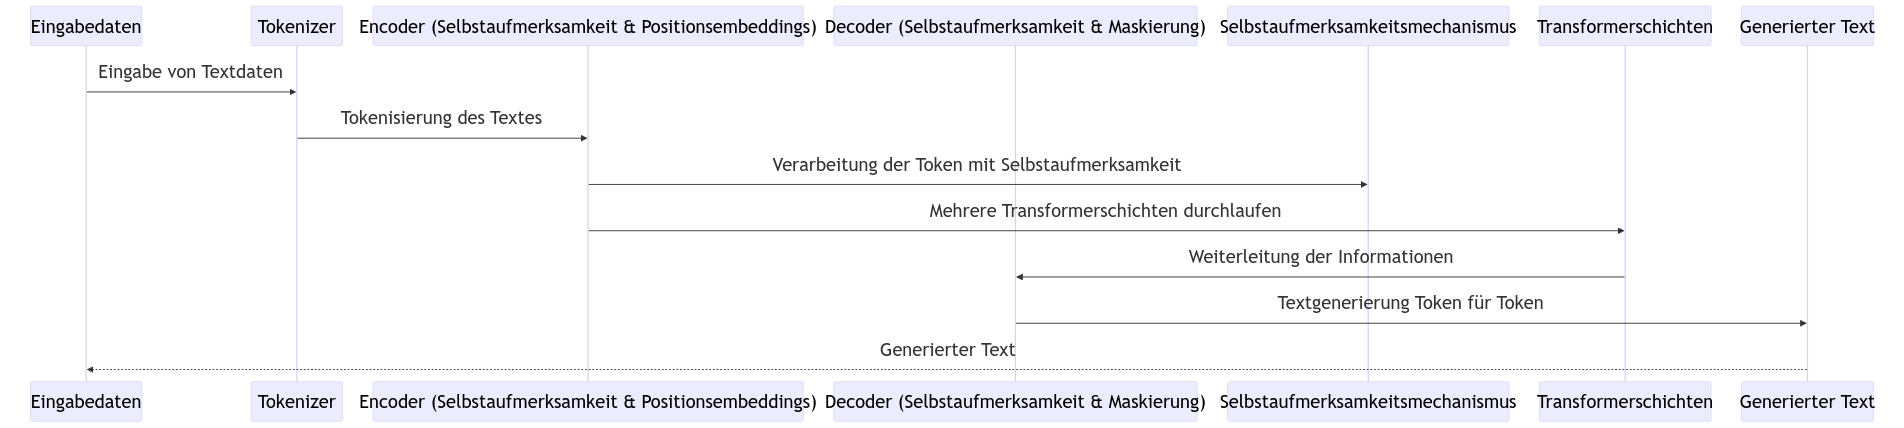
\includegraphics[width=1.0\textwidth]{gpt.png}
    \caption{Funktionsweise von Generative Pre-trained Transformer (GPT)\cite{yenduri_gpt_2024}}
    \label{fig:enter-label}
\end{figure*}

Generative Pre-trained Transformer (GPT) können sowohl Sprache verstehen als auch generieren. Diese Modelle können Aufgabenlisten interpretieren, Anweisungen befolgen, aus großen Mengen an Textdateien analysieren sowie Muster erkennen. Sie nutzen dafür Transformer-Architekturen, die sehr effizient sind und eine hohe Fähigkeit zur Handhabung von langen Kontextabhängigkeiten besitzen. Um die genannten Eigenschaften zu ermöglichen, waren zahlreiche technische Entwicklungen nötig.

Die Transformer-Architektur wurde ursprünglich von Vaswani et al. (2017) eingeführt. Sie basiert auf dem Mechanismus der Selbstaufmerksamkeit, der es ermöglicht, den Kontext jedes Wortes in einem Satz zu berücksichtigen, was besonders bei langen Texten von Vorteil ist\cite{brown_language_2020}.

Vortrainierte Sprachmodelle wie zum Beispiel GPT-3 basieren dabei auf der Transformer-Architektur und wurden durch Vortraining auf großen Datenmengen im Vergleich zu früheren GPT-Versionen verbessert. Dieses Vortraining ermöglicht es den Modellen, ein tiefes Verständnis der Sprache zu entwickeln, das durch Feinabstimmung auf spezifische Aufgaben weiter verfeinert werden kann.

Die Skalierung und Leistungsfähigkeit der GPT-Modelle korreliert stark mit der Anzahl der Parameter und der Menge der Trainingsdaten. OpenAI's GPT-3 hat dabei 175 Milliarden Parameter und wurde auf einer Vielzahl von Texten trainiert, was zu seiner hohen Leistungsfähigkeit beiträgt\cite{vaswani_attention_2023}.

Ein weiterer wichtiger Baustein im Kontext von GPTs ist das “Reinforcement Learning from Human Feedback (RLHF)”. Diese Technik wurde verwendet, um die Antworten der Modelle menschlicher und hilfreicher zu machen. Dabei lernen die Modelle aus menschlichem Feedback, wie sie auf verschiedene Anfragen reagieren sollen. OpenAI’s ChatGPT implementiert dies beispielsweise mit Hilfe deren Dialogsysteme.

Eine bedeutende Neuerung durch GPT-Modelle war das Zero-shot und Few-shot Learning\cite{kim_cot_2023}. GPT-Modelle haben dabei die Fähigkeit entwickelt, neue Aufgaben mit minimalem spezifischem Training zu lösen, was durch Zero-shot und Few-shot Learning erreicht wird. Dies bedeutet, dass sie Aufgaben lösen können, für die sie nicht explizit trainiert wurden, indem sie Beispiele aus dem Kontext ableiten\cite{brown_language_2020}.

Zusätzlich zu der Arbeit an den Sprachmodellen war der Fortschritt in der Hardware maßgeblich für den Erfolg von GPT. Insbesondere moderne GPUs und TPUs haben es ermöglicht, größere Modelle schneller und effizienter zu trainieren und auszuführen \cite{jeremy_training_2024}.

Diese technologischen Entwicklungen haben nicht nur die Effizienz und Leistungsfähigkeit von autonomen Agenten erhöht, sondern auch ihre Anwendungsfelder erweitert. Anwendungen reichen von automatisierten Kundendienstsystemen über persönliche Assistenten bis hin zu komplexen Analysewerkzeugen in verschiedenen wissenschaftlichen und industriellen Bereichen.

\subsection{Funktionsweise Autonomer KI-Agenten}

\begin{figure}[!htbp]
    \centering
    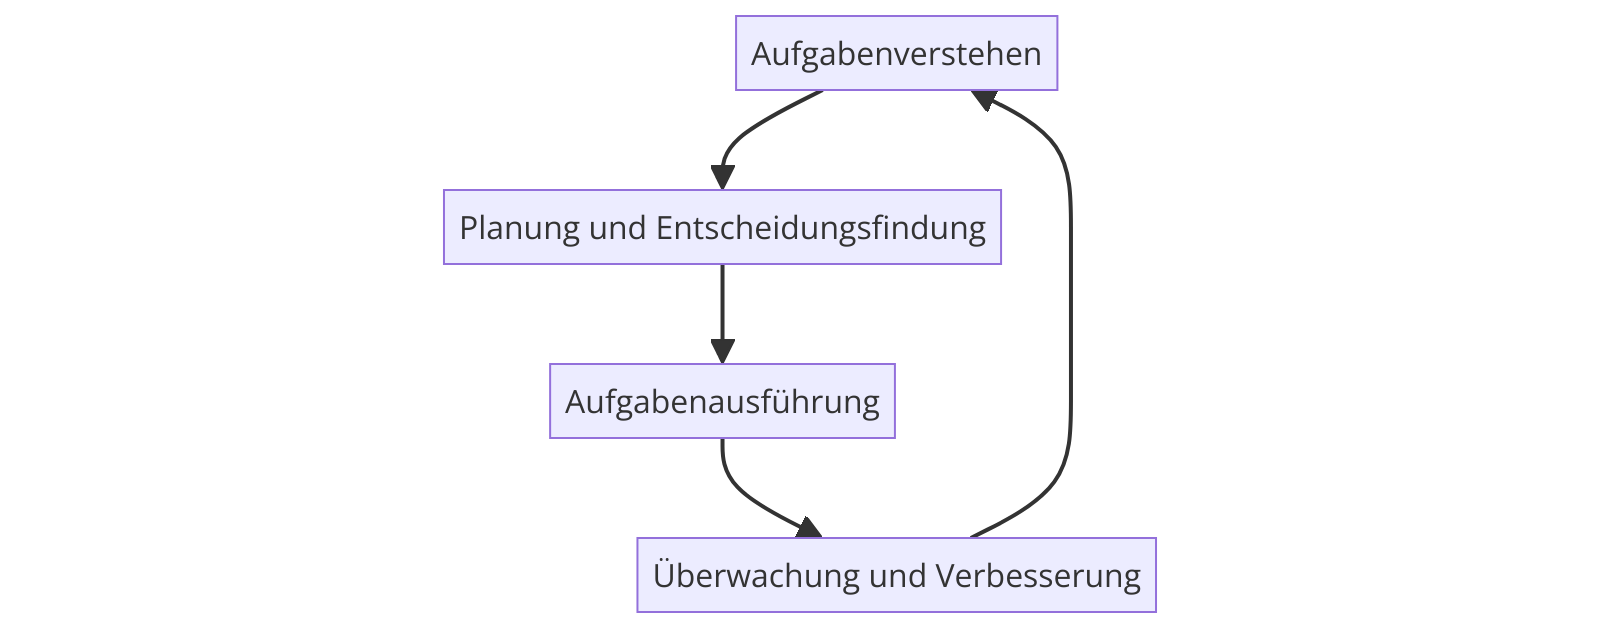
\includegraphics[width=0.6\textwidth]{prozess.png}
    \caption{Übersicht zur funktionsweise Autonomer KI-Agenten\cite{chu_240203628_nodate}}
    \label{fig:enter-label}
\end{figure}

Autonome KI-Agenten sind Systeme, die selbstständig Aufgaben ausführen können, ohne kontinuierliche menschliche Interaktion zu benötigen. Sie kombinieren fortgeschrittene Algorithmen, maschinelles Lernen und andere Technologien, um Entscheidungen zu treffen, Probleme zu lösen und Aktionen in dynamischen Umgebungen durchzuführen. Ein prominentes Beispiel für solche Agenten ist das bereits erwähnte AutoGPT\cite{significant_gravitas_autogpt_2024}, ein autonomer Agent, der auf dem beschriebenen GPT (Generative Pre-trained Transformer) basiert. Autonome KI-Agenten nutzen dabei vier grundlegende Schritte zur Automatisierung von Aufgaben: das Verständnis der Aufgabenstellung, die Planung und Entscheidungsfindung, die Durchführung der Aufgabe und die kontinuierliche Überwachung und Verbesserung der eigenen Handlungen.

Autonome KI-Agenten nutzen fortschrittliche Natural Language Processing (NLP) Techniken, um Eingaben zu verstehen. Diese Techniken ermöglichen es ihnen, Anweisungen in natürlicher Sprache zu interpretieren und die Intention des Nutzers zu erfassen. Die Fähigkeit zur Aufgabenverständnis basiert auf vortrainierten Sprachmodellen wie GPT-3, das durch umfangreiches Training auf großen Textdatensätzen ein tiefes Verständnis für Sprache und Kontext entwickelt hat\cite{barua_exploring_2024}.

Nach dem Verständnis der Aufgabenstellung verwenden autonome Agenten Algorithmen zur Planung und Entscheidungsfindung. Diese Algorithmen bewerten mögliche Aktionen und wählen diejenige aus, die am besten geeignet ist, die gewünschte Aufgabe zu erfüllen. Techniken wie Reinforcement Learning (RL) helfen dabei, durch Trial-and-Error zu lernen und optimale Strategien zu entwickeln. Das Modell wird durch Belohnungen und Bestrafungen für verschiedene Aktionen trainiert, um seine Entscheidungsfähigkeit zu verbessern\cite{chu_240203628_nodate}.

Einmal entschieden, welche Aktion ausgeführt werden soll, setzen autonome Agenten diese Entscheidung in die Tat um. Dies kann durch die Interaktion mit Software-APIs, Datenbanken oder direkt mit physischen Geräten geschehen. Beispiel: Ein KI-Agent könnte eine API nutzen, um Informationen aus einer Datenbank abzurufen, oder eine E-Mail automatisch senden, basierend auf vorher festgelegten Regeln und Kontextinformationen\cite{hague_multimodality_2024}.

Autonome Agenten überwachen kontinuierlich ihre eigenen Handlungen und ihre Ergebnisse. Durch Mechanismen wie Feedback-Schleifen und Fehlererkennung können sie ihre Strategien anpassen und verbessern. Hier kommt das Konzept des 'Reinforcement Learning from Human Feedback (RLHF)' ins Spiel, bei dem der Agent aus menschlichem Feedback lernt und seine Aktionen entsprechend anpasst, um menschlichere und hilfreichere Antworten zu liefern\cite{barua_exploring_2024}.

\subsection{Aktuelle technologische Entwicklungen}

Der Bereich der autonomen KI-Agenten ist hochaktuell und entwickelt sich rasant. Diese Dynamik wird durch die Vielzahl an laufenden Projekten deutlich, die unterschiedliche Ansätze und Anwendungen verfolgen. Derzeit existiert kein einheitlicher Standard oder ein bestimmtes Projekt, das als Status Quo bezeichnet werden könnte. Dies liegt unter anderem daran, dass autonome KI-Agenten auf verschiedene Anwendungsfälle spezialisiert werden können und daher eine breite Vielfalt an Implementationen und Spezialisierungen existiert. Im Folgenden werden verschiedene Typen und Anwendungsbereiche autonomer KI-Agenten vorgestellt, um einen umfassenden Überblick über den aktuellen Stand der Technik und die Vielfalt der Einsatzmöglichkeiten zu geben.

\subsubsection{Auto-GPT}
Autonomes System zur Aufgabenplanung und -ausführung: Auto-GPT nutzt fortschrittliche Sprachmodelle wie GPT-4, um autonome Aufgabenplanung und -ausführung zu ermöglichen. Dieses System kann eigenständig Aufgaben identifizieren, priorisieren und durchführen, basierend auf den Eingaben und Zielen des Benutzers. Auto-GPT integriert sich nahtlos mit verschiedenen APIs und Diensten, um umfassende Workflow-Automatisierung und Datenverarbeitung zu realisieren\cite{significant_gravitas_autogpt_2024}.

\subsubsection{AgentGPT}
Erweiterte Version von Auto-GPT mit zusätzlichen Funktionen: AgentGPT erweitert die Funktionalitäten von Auto-GPT durch die Implementierung zusätzlicher Features wie fortgeschrittene Kontextverarbeitung, Multi-Turn-Dialogfähigkeit und verbesserte Selbstoptimierungsmechanismen. Diese Verbesserungen ermöglichen eine noch präzisere und effizientere Aufgabenbearbeitung sowie eine bessere Nutzerinteraktion\cite{noauthor_reworkdagentgpt_nodate}.

\subsubsection{Devika}
Fortschrittlicher autonomer KI-Agent für die Softwareentwicklung: Devika ist ein fortschrittlicher KI-Agent, der hochrangige menschliche Anweisungen versteht, in detaillierte Schritte zerlegt, relevante Informationen recherchiert und den erforderlichen Code schreibt. Sie nutzt große Sprachmodelle, Planungs- und Argumentationsalgorithmen sowie Web-Browsing-Fähigkeiten. Devika zielt darauf ab, die Softwareentwicklung zu revolutionieren, indem sie als AI-Pair-Programmierer komplexe Aufgaben mit minimaler menschlicher Anleitung übernimmt. Dies umfasst das Erstellen neuer Funktionen, das Beheben von Fehlern oder die Entwicklung ganzer Projekte von Grund auf.\cite{noauthor_stitionaidevika_2024}.

\subsubsection{Copilot}
Assistenzsystem zur Unterstützung bei der Softwareentwicklung: Copilot, entwickelt von GitHub in Zusammenarbeit mit OpenAI, ist ein Assistenzsystem, das Softwareentwickler durch die automatische Generierung von Code unterstützt. Basierend auf den Eingaben des Entwicklers bietet Copilot Vorschläge für Code-Snippets, Funktionen und sogar komplette Algorithmen. Dieses System nutzt fortschrittliche Sprachmodelle, um den Kontext des Projekts zu verstehen und relevante Vorschläge zu machen, was die Produktivität und Effizienz erheblich steigert\cite{noauthor_github_2024}.

\section{Historische Entwicklung}
\subsection{Frühe Konzepte und theoretische Grundlagen}
Die Geschichte der künstlichen Intelligenz (KI) und der KI-Agenten reicht bis in die Mitte des 20. Jahrhunderts zurück. Frühe Konzepte wurden von Pionieren wie Alan Turing und John McCarthy entwickelt. Turing stellte in seinem berühmten Artikel "Computing Machinery and Intelligence" (1950) die Frage, ob Maschinen denken können, und führte den Turing-Test ein, der bis heute als Maßstab für maschinelle Intelligenz dient. John McCarthy prägte den Begriff 'künstliche Intelligenz' und war maßgeblich an der Organisation der Dartmouth Conference von 1956 beteiligt, die als Geburtsstunde der KI-Forschung gilt \cite{moto-oka_overview_1983}.
\cite{dagher_evolution_2023}

In den 1960er und 1970er Jahren wurden grundlegende Theorien und Modelle entwickelt, die den Weg für spätere Fortschritte ebneten. Ein bedeutendes Konzept aus dieser Zeit ist das von Marvin Minsky und Seymour Papert entwickelte "Perceptron", ein frühes Modell künstlicher neuronaler Netze. Diese theoretischen Grundlagen legten den Grundstein für die Entwicklung von KI-Agenten, die in der Lage sind, autonom zu agieren und Entscheidungen zu treffen\cite{leusin_evolutionary_2021}.

\subsection{Meilensteine in der Entwicklung autonomer Systeme}
Die Entwicklung autonomer Systeme hat mehrere bedeutende Meilensteine erreicht. Ein früher Meilenstein war die Entwicklung des Shakey-Roboters am Stanford Research Institute in den späten 1960er Jahren. Shakey war der erste Roboter, der mithilfe eines komplexen Regelwerks autonom navigieren und einfache Aufgaben ausführen konnte\cite{moto-oka_overview_1983}.

In den 1990er Jahren führte die DARPA (Defense Advanced Research Projects Agency) den Grand Challenge-Wettbewerb ein, bei dem autonome Fahrzeuge eine schwierige Strecke durch die Wüste navigieren mussten. Diese Wettbewerbe beschleunigten die Forschung und Entwicklung im Bereich der autonomen Fahrzeuge erheblich\cite{moto-oka_overview_1983}.

Ein weiterer Meilenstein war der Sieg von IBM's Watson im Jahr 2011 in der Quizshow "Jeopardy!". Watson konnte mithilfe fortschrittlicher Algorithmen und großer Datenmengen menschliche Gegner besiegen, was ein bedeutender Durchbruch in der Verarbeitung natürlicher Sprache war\cite{moto-oka_overview_1983}\cite{huang_history_2006}.

\subsection{Evolution der Hardware- und Softwaretechnologien}

Die Fortschritte in der Hardware- und Softwaretechnologie haben die Entwicklung von KI-Agenten maßgeblich beeinflusst. In den Anfangsjahren der KI-Forschung waren die Computer groß, teuer und hatten begrenzte Rechenleistung. Mit der Zeit wurden Computer jedoch kleiner, leistungsfähiger und kostengünstiger\cite{moto-oka_overview_1983}.

\subsubsection{Hardware-Evolution}
Ein bedeutender Fortschritt in der Hardwaretechnologie war die Entwicklung von spezialisierten Prozessoren wie GPUs (Graphics Processing Units), die für die parallele Verarbeitung großer Datenmengen optimiert sind. Diese Prozessoren haben die Leistungsfähigkeit von KI-Algorithmen erheblich verbessert und die Verarbeitung großer neuronaler Netze ermöglicht\cite{moto-oka_overview_1983}.

\subsubsection{Software-Evolution}
Auf der Softwareseite haben sich die Algorithmen und Frameworks zur Entwicklung von KI-Agenten weiterentwickelt. In den 1980er und 1990er Jahren wurden grundlegende Algorithmen wie Entscheidungsbäume und regelbasierte Systeme entwickelt. In den letzten Jahrzehnten haben maschinelles Lernen und tiefe neuronale Netze die KI-Forschung revolutioniert. Frameworks wie TensorFlow und PyTorch haben die Entwicklung und Implementierung von KI-Modellen vereinfacht und beschleunigt\cite{moto-oka_overview_1983}.

TensorFlow ist ein von Google entwickeltes Open-Source-Framework für maschinelle Intelligenz, das eine flexible Plattform für maschinelles Lernen und tiefe neuronale Netze bietet. Es erleichtert Entwicklern das Erstellen, Trainieren und Deployen von Modellen und unterstützt vielfältige Einsatzmöglichkeiten.
\cite{noauthor_161001178_nodate}

PyTorch ist ein von Facebook entwickeltes Open-Source-Framework, das für seine Benutzerfreundlichkeit und Flexibilität geschätzt wird. Es unterstützt dynamische Berechnungsgrafen, was das Experimentieren und Testen neuer Modelle erleichtert, und wird von einer wachsenden Community weiterentwickelt\cite{noauthor_pytorch_nodate}.

Zusammenfassend lässt sich sagen, dass die historische Entwicklung von KI-Agenten von frühen theoretischen Konzepten und grundlegenden Modellen bis hin zu praktischen Anwendungen und bedeutenden Meilensteinen reicht. Fortschritte in der Hardware- und Softwaretechnologie haben diese Entwicklung vorangetrieben und die Grundlage für die modernen KI-Agenten gelegt, die wir heute kennen. Mit fortschreitender Technologie und Forschung wird die Rolle von KI-Agenten in unserem täglichen Leben weiter zunehmen und neue Möglichkeiten und Herausforderungen mit sich bringen\cite{moto-oka_overview_1983}.

\subsection{Historische Entwicklung anhand von Beispielen}

\begin{table*}[h!]
    \centering
    \begin{tabularx}{\textwidth}{|p{0.8cm}|X|X|X|} \hline 
         & Input & Verarbeitung & Output \\ \hline 
         Clippy & Benutzeraktionen in Microsoft Office, explizite Hilfeanforderungen & Kontextbezogene Hilfe durch Beobachtung und Analyse, Erkennung von Phrasen wie 'Sehr geehrter' und 'Mit freundlichen Grüßen' & Anzeigen von Tipps, Präsentation relevanter Hilfethemen, Vorschläge im Office-Interface \\ \hline 
         Siri & Sprach- oder Tastatureingaben & Umwandlung von Sprache in Text, Kontext- und Bedeutungsanalyse, Zugriff auf Datenbanken und Online-Server & Natürliche Sprache Antworten, Ausführen angeforderter Aktionen wie Nachrichten senden oder Apps öffnen \\ \hline 
         Duplex & Sprachbefehle an Google Assistant & Umwandlung von Sprache in Text, Extraktion wichtiger Informationen, Nutzung von neuronalen Netzwerken für Sprachverarbeitung & Führt Telefonanrufe durch, interagiert natürlich mit Unternehmen, bestätigt Reservierungen und Termine \\ \hline 
         Auto GPT & Detaillierte Beschreibung der Agentenrolle, Liste von Zielen & Erstellung eines System-Prompts, Generierung von Aktionen basierend auf Kontext, iterativer Zyklus von Denken, Handeln und Beobachten & Durchführung von Websuchen, Ausführung von Code, Verwaltung von Dateien, Erstellung von Berichten \\ \hline
    \end{tabularx}
    \caption{Übersicht zur Funktionsweise verschiedener KI-Agenten}
\end{table*}

Um die Entwicklung und Funktionsweise dieser Systeme besser zu verstehen, haben wir in diesem Text exemplarisch vier bedeutende KI-Systeme ausgewählt: Clippy, Siri, Google Duplex und Auto-GPT. Diese Beispiele wurden gewählt, um die Evolution der KI-Technologien zu veranschaulichen, beginnend mit frühen Versuchen, benutzerfreundliche Schnittstellen zu schaffen, bis hin zu modernen, hochentwickelten Systemen, die komplexe und autonome Aufgaben ausführen können.

Der nachfolgende Abschnitt beleuchtet die Kernfrage, wie unterschiedliche KI-Systeme mit Benutzerinteraktionen umgehen und wie sie diese verarbeiten, um relevante und hilfreiche Ausgaben zu generieren. Diese Frage ist zentral, da sie die Effizienz, Nützlichkeit und Benutzerakzeptanz der KI-Systeme beeinflusst. Durch die Analyse der Eingabe (Input), der Verarbeitung und der Ausgabe (Output) können wir die Stärken und Schwächen der verschiedenen Systeme erkennen und besser verstehen, wie sie ihre Ziele erreichen.

Als Vergleichsvariablen wurden Input, Verarbeitung und Output gewählt, da diese drei Aspekte die grundlegenden Komponenten der Funktionsweise eines jeden KI-Systems darstellen. Der Input beschreibt, wie Benutzer mit dem System interagieren und welche Art von Daten oder Befehlen sie eingeben. Die Verarbeitung beleuchtet die internen Mechanismen und Algorithmen, die das System verwendet, um den Input zu interpretieren und darauf zu reagieren. Der Output zeigt, welche Art von Unterstützung, Information oder Aktion das System schließlich dem Benutzer bietet.

 
\subsubsection{Clippy}
Clippy, auch bekannt als der 'Office Assistant', wurde von Microsoft Mitte der 1990er Jahre entwickelt, um Benutzern bei der Nutzung von Microsoft Office zu helfen. Die Idee hinter Clippy entstand aus dem Forschungsprojekt Microsoft Bob, einem Versuch, eine benutzerfreundlichere Schnittstelle für Windows 95 zu schaffen. Microsoft Bob war ein Overlay, das Nutzern durch animierte Charaktere wie Clippy Unterstützung bieten sollte. Obwohl Bob schnell eingestellt wurde, lebte die Idee eines virtuellen Assistenten weiter.

Clippy selbst wurde erstmals 1997 mit Office 97 eingeführt und sollte durch Beobachtung und Analyse von Benutzeraktivitäten kontextbezogene Hilfe anbieten. Das Design von Clippy wurde durch Studien von Stanford-Professoren wie Byron Reeves und Clifford Nass beeinflusst, die entdeckten, dass Menschen Computer ähnlich wie andere Menschen behandeln\cite{noauthor_media_nodate}.

\paragraph{Input}Benutzer interagieren mit dem virtuellen Assistenten, indem sie Aktionen in Microsoft Office ausführen oder explizit um Hilfe bitten. Dies geschieht durch Mausklicks, Tastatureingaben oder Office-Befehle, die den Assistenten aufrufen.
\paragraph{Verarbeitung} Anhand vordefinierter Algorithmen und Heuristiken werden Benutzeraktivitäten mit möglichen Absichten abgeglichen. Die Erkennung von Phrasen wie „Sehr geehrter“ oder „Mit freundlichen Grüßen“ löst Vorschläge für das Schreiben eines Briefes aus. Dieser Entscheidungsprozess basiert auf einer Datenbank mit häufigen Aufgaben und Benutzeranfragen in Microsoft Office.
\paragraph{Output}Der Assistent bietet Unterstützung, indem er Tipps anzeigt, relevante Hilfethemen präsentiert oder direkt im Office-Interface Aktionen vorschlägt. Wenn das Programm beispielsweise einen Brief erkennt, könnten Formatierungstipps oder eine Vorlage vorgeschlagen werden. Benutzer können auf die Vorschläge reagieren, die angebotene Hilfe annehmen oder ablehnen. Die Antworten sind so gestaltet, dass sie einem menschlichen Assistenten ähneln und hilfreich sein sollen\cite{cain_life_2017}.
 
\subsubsection{Siri}
Siri begann als Projekt von SRI International, das aus einer DARPA-Initiative hervorging und ursprünglich als CALO (Cognitive Assistant that Learns and Organizes) entwickelt wurde. Siri wurde später als Startup gegründet und schließlich von Apple übernommen. Apple integrierte Siri in das iPhone, fügte Funktionen hinzu und verbesserte die Benutzerfreundlichkeit. Dabei werden folgende Funktionsweisen verwendet:
\paragraph{Input} Der Benutzer gibt eine Anfrage per Sprache oder Tastatur ein. Siri zeichnet die Stimme auf und wandelt die Schallwellen in digitale Daten um.
\paragraph{Verarbeitung} Die digitalen Daten werden in Text umgewandelt. Im Hintergrund werden Muster, Phrasen und Schlüsselwörter identifiziert um mit Algorithmen, den Kontext und die Bedeutung zu verstehen. Siri greift auf interne Datenbanken und Online-Server zu, um die benötigten Informationen zu finden. 
\paragraph{Output} Mit den gefundenen Daten werden vollständige und relevante Sätze basierend auf der Anfrage erstellt.  Dadurch kann die Antwort in natürlicher Sprache zurück gegeben werden oder die angeforderte Aktion, wie das Senden einer Nachricht oder das Öffnen einer App ausgeführt werden.
\cite{noauthor_voice_nodate}
\cite{noauthor_hey_nodate}
 
\subsubsection{Google Duplex}
Google Duplex wurde 2018 vorgestellt und ist eine fortschrittliche Technologie, die darauf abzielt, natürliche Gespräche mit Computern zu ermöglichen, insbesondere für Aufgaben wie das Vereinbaren von Terminen. Die Technologie wurde entwickelt, um die Interaktion mit automatisierten Systemen menschlicher und intuitiver zu gestalten. Duplex nutzt fortschrittliche KI-Technologien, um menschliche Sprache und Verhaltensmuster nachzuahmen. Dabei kommen neuronale Netzwerke und maschinelles Lernen zum Einsatz, um die Sprachverarbeitung und Antwortgenerierung zu verbessern.

\paragraph{Input} Der Benutzer beginnt die Interaktion, indem er einen Sprachbefehl an den Google Assistant richtet, zum Beispiel „Reserviere einen Tisch für Freitagabend in einem italienischen Restaurant“. Dieser Befehl wird durch die Google Assistant App erfasst und an Google Duplex weitergeleitet, das die Aufgabe übernimmt.

\paragraph{Verarbeitung} Sobald der Befehl erfasst wurde, wird er durch Google’s Automatic Speech Recognition (ASR) System in Text umgewandelt. Duplex analysiert diesen Text, um wichtige Informationen wie Datum, Uhrzeit und Ort der Reservierung zu extrahieren. Es berücksichtigt auch den Verlauf des Gesprächs und andere Kontextinformationen, um die Anfrage genau zu verstehen. Hierfür verwendet Duplex ein rekurrentes neuronales Netzwerk (RNN), das auf umfangreichen Datensätzen von Telefongesprächen trainiert wurde. Dieses Netzwerk nutzt TensorFlow Extended (TFX) zur Optimierung und bewältigt die Komplexität natürlicher Sprache.

Auf Basis der Analyse generiert Duplex eine Antwort, die durch ein Text-to-Speech-System in natürliche Sprache umgewandelt wird. Dabei werden Techniken wie WaveNet eingesetzt, um Intonation und Betonung menschlich klingen zu lassen.

\paragraph{Output} Duplex führt dann den Anruf beim gewünschten Unternehmen durch und führt das Gespräch, als wäre es eine echte Person. Es fragt nach verfügbaren Zeiten und bestätigt die Reservierung oder den Termin basierend auf den Präferenzen des Benutzers. Während des Gesprächs kann Duplex auf Unterbrechungen, Rückfragen und spontane Änderungen reagieren, um eine nahtlose und natürliche Konversation zu gewährleisten.

Nach Abschluss des Anrufs informiert Duplex den Benutzer über den Ausgang des Gesprächs und bestätigt die Details der Reservierung oder des Termins. Google Duplex hebt sich durch seine Fähigkeit hervor, natürliche und kontextbewusste Gespräche zu führen, die weit über die Möglichkeiten herkömmlicher Sprachassistenten hinausgehen.
\cite{noauthor_google_nodate}

\subsubsection{Auto-GPT}
Auto-GPT wurde als experimentelles Open-Source-Projekt entwickelt, das die Fähigkeiten von GPT-4 nutzt, um vollständig autonome Aufgaben durchzuführen. Das Projekt baut auf der Architektur und den Modellen von OpenAI auf und erweitert diese, um eigenständig Ziele zu erreichen, die in natürlicher Sprache definiert werden. Auto-GPT führt selbstständig Aktionen aus, indem es größere Aufgaben in kleinere Teilaufgaben zerlegt und diese nacheinander abarbeitet.

\paragraph{Input} Der Benutzer startet den Prozess, indem er eine detaillierte Beschreibung der Rolle des AI-Agenten und eine Liste von Zielen vorgibt. Zum Beispiel könnte der Benutzer einen AI-Agenten namens "ResearchGPT" definieren, dessen Aufgabe es ist, Marktforschung zu betreiben, mit spezifischen Zielen wie das Finden der besten Produkte auf dem Markt und das Erstellen von Berichten. \cite{noauthor_papers_nodate}

\paragraph{Verarbeitung} Die Verarbeitung in Auto-GPT erfolgt in mehreren Schritten. Zunächst erstellt Auto-GPT einen System-Prompt, der die Ziele und die Beschreibung des Agenten enthält. Dieser System-Prompt definiert auch die verfügbaren Ressourcen, die Befehle, die der Agent verwenden kann, und die Einschränkungen, die er beachten muss. Der aktuelle Kontext wird basierend auf der Benutzereingabe, dem bisherigen Chat-Verlauf und relevanten gespeicherten Erinnerungen (z.B. Ergebnisse früherer Befehle) konstruiert. Dies stellt sicher, dass der Agent immer die notwendigen Informationen zur Verfügung hat, um fundierte Entscheidungen zu treffen. Auto-GPT verwendet die OpenAI-API, um basierend auf dem aktuellen Kontext Vorschläge für die nächste Aktion zu generieren. Diese Vorschläge werden in einem Zyklus von Denken, Handeln und Beobachten verarbeitet, wobei der Agent selbstkritisch sein eigenes Verhalten bewertet und verbessert. Die Ergebnisse jeder Aktion werden in einem externen Speichersystem (z.B. eine Datenbank oder eine Datei) gespeichert und bei Bedarf abgerufen, um den Kontext für zukünftige Aktionen zu bereichern und zu verfeinern. \cite{rima_rimabuildsautogpt-handbook_2024}

\paragraph{Output} Auto-GPT liefert Ergebnisse in mehreren Formen. Der Agent kann Befehle ausführen, wie das Durchführen von Websuchen, das Ausführen von Code oder das Verwalten von Dateien. Zum Beispiel könnte der Agent eine Websuche durchführen, um Informationen zu sammeln, und die Ergebnisse in einem Bericht speichern. Nach Abschluss einer oder mehrerer Aufgaben erstellt der Agent einen umfassenden Bericht, der die Ergebnisse und Empfehlungen basierend auf den gesammelten Daten enthält. Der Agent informiert den Benutzer kontinuierlich über den Fortschritt und die Ergebnisse seiner Aktionen. Bei Bedarf kann der Benutzer zusätzliche Anweisungen geben oder den Agenten anweisen, spezifische Befehle auszuführen. Durch diese autonome und iterative Vorgehensweise kann Auto-GPT komplexe Aufgaben effizient und selbstständig bewältigen, was es zu einem mächtigen Werkzeug für verschiedenste Anwendungen macht.
\cite{noauthor_papers_nodate}

\section{Agentensysteme}

Agentensysteme, auch bekannt als KI-Agenten, sind intelligente Systeme, die darauf ausgelegt sind, autonom zu agieren, Entscheidungen zu treffen und Aufgaben zu erfüllen, die traditionell menschliches Eingreifen erfordern. Diese Systeme können eigenständige Entscheidungen treffen, komplexe Aufgaben lösen und in vielfältigen Umgebungen agieren. Die Entwicklung solcher Agenten hat bedeutende Fortschritte in der Robotik, im maschinellen Lernen und in der künstlichen Intelligenz hervorgebracht und bietet Potenzial für zahlreiche Branchen, von der industriellen Automatisierung und der Logistik bis hin zu Gesundheitswesen, Finanzdienstleistungen und dem autonomen Fahren \cite{v-hanki_was_2023}.

\subsection{Anfänge und Limitationen}
Die Entwicklung von Agentensystemen begann mit einfachen regelbasierten Systemen, die auf vordefinierten Regeln und Logiken basierten. Diese frühen Systeme waren limitiert in ihrer Fähigkeit, komplexe Aufgaben zu bewältigen oder aus Erfahrungen zu lernen. Mit Fortschritten im maschinellen Lernen und der künstlichen Intelligenz haben sich jedoch die Fähigkeiten dieser Systeme erheblich verbessert. Moderne KI-Agenten können aus Daten lernen, ihre Strategien anpassen und sich an neue Umgebungen und Herausforderungen anpassen. Trotz dieser Fortschritte gibt es weiterhin Limitationen, insbesondere in Bezug auf die Interpretierbarkeit ihrer Entscheidungen und die Notwendigkeit großer Datenmengen für effektives\cite{kwasny_overcoming_1990} 

\subsection{Klassifikation und Arten von Agenten}
KI-Agenten lassen sich in verschiedene Kategorien einteilen, basierend auf ihren Fähigkeiten und der Art und Weise, wie sie mit ihrer Umgebung interagieren. Im Folgenden werden die drei Hauptkategorien reaktive Agenten, kognitive Agenten und hybride Agenten beschrieben, die in der Forschung und Anwendung besonders hervorgehoben werden. 

\subsubsection{Reaktive Agenten}
Reaktive Agenten reagieren auf spezifische Eingaben oder Umgebungsreize mit vorgegebenen Aktionen. Sie verfügen über keine Gedächtnisfunktion und können daher keine langfristigen Strategien entwickeln. Ein klassisches Beispiel für reaktive Agenten sind einfache Chatbots, die auf vordefinierte Schlüsselwörter reagieren. Diese Agenten sind auf unmittelbare Reaktionen beschränkt und eignen sich besonders für Anwendungen, die schnelle und einfache Antworten erfordern\cite{kwasny_overcoming_1990} 

\subsubsection{Kognitive Agenten}
Kognitive Agenten sind komplexer und leistungsfähiger als reaktive Agenten. Sie verfügen über eine Gedächtnisfunktion und können auf Basis von gesammelten Erfahrungen und Daten langfristige Strategien entwickeln. Diese Agenten nutzen maschinelles Lernen und fortschrittliche Algorithmen, um ihre Entscheidungen zu optimieren. Beispiele für kognitive Agenten sind fortgeschrittene virtuelle Assistenten, die in der Lage sind, komplexe Anfragen zu verarbeiten und personalisierte Empfehlungen zu geben\cite{megherbi_hybrid_2012}

\subsubsection{Hybride Agenten}
Hybride Agenten kombinieren die Eigenschaften von reaktiven und kognitiven Agenten. Sie können sowohl auf spezifische Reize reagieren als auch aus Erfahrungen lernen und langfristige Strategien entwickeln. Diese Flexibilität macht sie besonders nützlich für komplexe Anwendungen, bei denen schnelle Reaktionen und strategisches Denken erforderlich sind. Ein Beispiel für hybride Agenten sind moderne E-Commerce-Systeme, die Kunden in Echtzeit unterstützen und gleichzeitig aus deren Verhalten lernen, um zukünftige Empfehlungen zu optimieren\cite{megherbi_hybrid_2012}

\subsection{Abgrenzung: Software/Virtuelle vs. Roboter Autos}
Es ist wichtig, zwischen verschiedenen Typen von Agentensystemen zu unterscheiden:

\subsubsection{Software/Virtuelle Agenten}
Diese Agenten operieren in virtuellen oder digitalen Umgebungen. Sie sind reine Softwarelösungen, die beispielsweise als Chatbots, virtuelle Assistenten oder Empfehlungsalgorithmen in E-Commerce-Plattformen fungieren. Sie interagieren hauptsächlich durch digitale Schnittstellen und sind darauf ausgelegt, textbasierte oder datenbasierte Aufgaben zu erfüllen\cite{v-hanki_was_2023}.

\subsubsection{Physische Agenten (Roboter Autos)}
Physische Agenten hingegen sind in der realen Welt tätig. Dazu gehören autonome Roboter und Fahrzeuge, die in physischen Umgebungen agieren und mit der realen Welt interagieren. Diese Agenten müssen nicht nur kognitive Fähigkeiten besitzen, sondern auch in der Lage sein, physische Aktionen auszuführen. Beispiele sind Industrieroboter, die in Fabriken arbeiten, und autonome Fahrzeuge, die im Straßenverkehr navigieren\cite{v-hanki_was_2023}.

\section{Anwendungsfelder}

Autonome KI-Agenten finden in zahlreichen Branchen und Anwendungen Einsatz, indem sie ihre Fähigkeit zur selbstständigen Entscheidungsfindung und Problemlösung nutzen. Im Folgenden werden verschiedene Anwendungsszenarien vorgestellt

\subsection{Gesundheitswesen}

Im Gesundheitswesen unterstützen KI-Agenten bei der Diagnose, Behandlung und Verwaltung von Patienteninformationen. Ein prominentes Beispiel ist IBM Watson, das Ärzten hilft, Krebsdiagnosen zu stellen und Behandlungspläne basierend auf umfangreichen medizinischen Datenbanken und aktuellen Forschungsergebnissen zu empfehlen\cite{somashekhar_watson_2018}. Diese KI-Agenten analysieren Patientendaten, um personalisierte Behandlungspläne zu erstellen und die Entscheidungsfindung im Gesundheitswesen zu verbessern. KI im Gesundheitswesen stellt einen Paradigmenwechsel dar, da sie durch die zunehmende Verfügbarkeit von Gesundheitsdaten und den schnellen Fortschritt der Analysetechniken ermöglicht wird. Künstliche Intelligenz kann auf verschiedene Arten von Gesundheitsdaten angewendet werden, sowohl strukturiert als auch unstrukturiert. Zu den beliebten KI-Techniken gehören maschinelles Lernen für strukturierte Daten, wie die klassische Support-Vektor-Maschine und neuronale Netze, sowie das moderne Deep Learning und die Verarbeitung natürlicher Sprache für unstrukturierte Daten. Wichtige Krankheitsbereiche, die KI-Tools verwenden, umfassen Krebs, Neurologie und Kardiologie. Beispielsweise werden in der Schlaganfallbehandlung KI-Anwendungen in den Bereichen Früherkennung und Diagnose, Behandlung sowie Vorhersage von Ergebnissen und Prognosebewertung eingesetzt\cite{jiang_artificial_2017}.

Ein konkretes Beispiel für den Einsatz von KI im Bereich der Onkologie ist das System Watson for Oncology (WFO). In einer Studie mit 638 Brustkrebspatienten am Manipal Comprehensive Cancer Center in Bengaluru, Indien, wurden die Behandlungsempfehlungen von WFO und einem multidisziplinären Tumorboard verglichen. Die Ergebnisse zeigten eine hohe Übereinstimmung (93\%) der Behandlungsempfehlungen zwischen WFO und dem Tumorboard. Die Analyse ergab, dass Patienten mit Stadium I oder IV weniger wahrscheinlich übereinstimmende Empfehlungen erhielten als Patienten mit Stadium II oder III. Das Alter der Patienten hatte ebenfalls einen signifikanten Einfluss auf die Übereinstimmung, während der Rezeptorstatus keinen Einfluss hatte. Diese Studie zeigt, dass WFO ein hilfreiches Werkzeug für die Entscheidungsfindung bei der Brustkrebsbehandlung sein kann, insbesondere an Zentren, an denen Expertenressourcen für Brustkrebs begrenzt sind\cite{somashekhar_watson_2018}.

\subsection{Finanzdienstleistungen}

Autonome KI-Agenten spielen eine wichtige Rolle in der Finanzbranche, insbesondere im Bereich der Betrugserkennung und des algorithmischen Handels. Banken und Finanzinstitute nutzen KI-Agenten, um Transaktionen in Echtzeit zu überwachen und verdächtige Aktivitäten zu erkennen\cite{mohanty_role_2023}. Durch den Einsatz von KI-basierten Technologien wie Teradata, Feedzai, Riskified und anderen konnten die Instanzen von Betrug erheblich reduziert und die Effizienz und Effektivität der Geschäftsabläufe gesteigert werden. Diese Technologien bieten den Finanzinstituten nicht nur einen Wettbewerbsvorteil, sondern tragen auch dazu bei, die Reputation der Banken zu wahren und zu verbessern. Darüber hinaus hat die Künstliche Intelligenz in der Finanz- und Bankdienstleistungsbranche die Betriebskosten gesenkt und die Geschäftsergebnisse verbessert.

AI hat das Asset Management revolutioniert, indem sie die Effizienz, Genauigkeit und Compliance in den Bereichen Portfoliomanagement, Handel und Risikomanagement verbessert hat\cite{bartram_artificial_2020}. Investmentfirmen und Hedgefonds nutzen KI-gesteuerte Handelsalgorithmen, um Marktanalysen durchzuführen und Handelsstrategien zu optimieren. Ein prominentes Beispiel ist die Firma Two Sigma, die algorithmische Handelsstrategien entwickelt und umsetzt. KI-Techniken helfen dabei, Portfolios basierend auf genaueren Risiko- und Renditeprognosen sowie komplexeren Einschränkungen zu konstruieren. Handelsalgorithmen verwenden KI, um neuartige Handelssignale zu entwickeln und Trades mit niedrigeren Transaktionskosten auszuführen. Außerdem verbessert KI das Risikomodell und die Prognose, indem sie Erkenntnisse aus neuen Datenquellen generiert. Trotz dieser Vorteile bringt die Nutzung von KI auch neue Risiken und Herausforderungen mit sich, wie die Komplexität der Modelle und die Abhängigkeit von der Datenintegrität.

\subsection{E-Commerce}

Im E-Commerce werden KI-Agenten zur Personalisierung des Einkaufserlebnisses eingesetzt. Plattformen wie Amazon und Alibaba nutzen KI-Agenten, um Kunden personalisierte Produktvorschläge zu machen, basierend auf ihrem Verhalten und ihren Präferenzen\cite{behera_personalized_2020}. Darüber hinaus helfen KI-Agenten bei der Optimierung der Preisgestaltung und der Bestandsverwaltung, indem sie Marktdaten analysieren und Nachfrageprognosen erstellen. Diese Anwendungen tragen dazu bei, die Kundenzufriedenheit zu erhöhen und die Umsätze zu steigern\cite{joshi_artificial_2024}.

Dazu werden KI-Agenten zur Personalisierung des Einkaufserlebnisses eingesetzt. Plattformen wie Amazon und Alibaba nutzen KI-Agenten, um Kunden personalisierte Produktvorschläge zu machen, basierend auf ihrem Verhalten und ihren Präferenzen. Diese Recommender Engines helfen, relevante Artikel anzubieten, die den Warenkorbwert verbessern und die Kundenbindung stärken. Eine experimentelle Studie in einem mittelgroßen Gesundheitsprodukte-Einzelhändler zeigte, dass die Einführung eines personalisierten Empfehlungssystems das durchschnittliche monatliche Umsatzwachstum um 33,49\%, den durchschnittlichen Bestellwert um 32,79\% und die Artikel pro Bestellung um 1,93\% steigerte. Dies verdeutlicht die signifikanten Vorteile personalisierter Marketinginformationen für den Kundenentscheidungsprozess\cite{behera_personalized_2020}.

Darüber hinaus helfen KI-Agenten bei der Optimierung der Preisgestaltung und der Bestandsverwaltung, indem sie Marktdaten analysieren und Nachfrageprognosen erstellen. Durch den Einsatz von Technologien wie maschinellem Lernen, natürlicher Sprachverarbeitung und prädiktiver Analytik können E-Commerce-Unternehmen ihre Abläufe optimieren und die Entscheidungsprozesse verbessern. KI-basierte Systeme tragen auch zur Betrugserkennung und zur Optimierung der Lieferkette bei, was zu effizienteren Betriebsabläufen und einer höheren Kundenzufriedenheit führt. Die Integration von KI in E-Commerce-Plattformen ermöglicht es Unternehmen, personalisierte Erlebnisse zu bieten und die Umsätze zu steigern, während gleichzeitig die betriebliche Effizienz verbessert wird\cite{misischia_chatbots_2022}.

\subsection{AutoGPT}

Der bereits erwähnte OpenAI wrapper AutoGPT ist ein autonomer KI-Agent, der auf dem GPT-4-Modell von OpenAI basiert und in der Lage ist, komplexe Aufgaben ohne menschliches Eingreifen zu bewältigen. AutoGPT kann durch das Zerlegen größerer Aufgaben in kleinere Teilaufgaben und deren iterative Bearbeitung eigenständige Entscheidungen treffen und Aktionen ausführen. Diese Technologie findet Anwendung in Bereichen wie Marktforschung, Projektmanagement und automatisierte Dokumentenerstellung. Ein Beispiel für den Einsatz von AutoGPT ist das autonome Management von Social-Media-Konten, bei dem der Agent Inhalte erstellt, plant und veröffentlicht sowie auf Interaktionen reagiert. Dies zeigt das Potenzial von AutoGPT, Unternehmen und Einzelpersonen dabei zu unterstützen, ihre Online-Präsenz zu verbessern, ein breiteres Publikum zu erreichen und ihre Social-Media-Ziele zu verwirklichen\cite{pogla_ultimate_2024}. Durch kontinuierliche Optimierung und Anpassung der Strategien auf Basis der von AutoGPT generierten Einblicke können Benutzer langfristig erfolgreich sein und sich im Wettbewerb behaupten.

Die Vielseitigkeit und Anpassungsfähigkeit von AutoGPT und anderen großen Sprachmodellen (LLMs) bieten eine Grundlage für die Entwicklung allgemeiner KI-Agenten, die in verschiedenen Szenarien eingesetzt werden können. Diese LLM-basierten Agenten sind in der Lage, ihre Umgebung zu erfassen, Entscheidungen zu treffen und Handlungen auszuführen, was sie zu potenziellen Kandidaten für die Verwirklichung von Artificial General Intelligence (AGI) macht. Eine umfassende Untersuchung zeigt, dass LLM-basierte Agenten in Einzel- und Multi-Agenten-Szenarien sowie in der Zusammenarbeit mit Menschen signifikante Fortschritte erzielt haben\cite{xi_rise_2023}. Beispielsweise wurde in einer vergleichenden Studie zwischen einem generativen KI-Modell wie GPT-4 und einem menschlichen Projektmanager festgestellt, dass beide unterschiedliche Stärken und Schwächen in der Projektplanung aufweisen und sich somit ergänzen können. Diese Synergie zwischen menschlicher Expertise und KI ermöglicht die Erstellung robuster und vertrauenswürdiger Projektpläne, wobei die Integration von menschlichen und KI-Fähigkeiten entscheidend ist, um das volle Potenzial der KI auszuschöpfen\cite{barcaui_who_2023}.

\subsection{Persönliche Assistenten}

Persönliche Assistenten, wie sie in der historischen Entwicklung vorgestellt wurden, bieten Benutzern personalisierte Unterstützung in ihrem täglichen Leben. Diese Assistenten können Aufgaben wie Terminplanung, Erinnerungen, Informationssuche und Kommunikation übernehmen. Ein prominentes Beispiel ist Apple's Siri, das Sprachbefehle verarbeitet und Aktionen wie das Senden von Nachrichten, das Erstellen von Kalenderereignissen und das Abrufen von Informationen aus dem Internet ausführt. Google Assistant und Amazon Alexa sind weitere Beispiele für persönliche Assistenten, die durch ihre Integration in Smart-Home-Geräte und andere Dienste eine nahtlose Benutzererfahrung bieten. Diese virtuellen Assistenten nutzen maschinelles Lernen und natürliche Sprachverarbeitung (NLP), um ihre Leistung zu optimieren und eine menschenähnliche Interaktion zu ermöglichen\cite{madhuri_survey_2020}.

Virtuelle Assistenten spielen eine immer wichtigere Rolle im Alltag und unterstützen bei vielfältigen Aufgaben wie Alarmen, Musikabspielen, Gesichtserkennung, Spracherkennung, handschriftlicher Erkennung, Erinnerungen, Antworten, Krankheitsdiagnosen und mehr. Sie werden in Bereichen wie Bildung, Medizin, Landwirtschaft, Medien, sozialen Netzwerken, selbstfahrenden Autos, Banken und Betrugserkennung eingesetzt. Durch maschinelles Lernen und künstliche neuronale Netze werden diese Assistenten trainiert, um Benutzer so genau wie möglich zu unterstützen. Beispielsweise ermöglicht ein sprachbefehlsgesteuerter AI-Assistent die Steuerung von Heimautomatisierungssystemen, das Versenden von E-Mails und WhatsApp-Nachrichten, die Durchführung von Google- und Wikipedia-Suchen sowie das Abspielen von Musik und Videos. Solche Assistenten können auch Wetter- und Nachrichtenaktualisierungen bereitstellen und die Leistung des Computers überwachen. Diese Technologien zeigen das Potenzial, die Effizienz und den Komfort im täglichen Leben der Benutzer erheblich zu steigern\cite{charan_home_2023}.

\section{Potenziale und Herausforderungen}

Die vorliegende Untersuchung befasst sich umfassend mit autonomen KI-Agenten, ihrer technologischen Entwicklung und ihren vielfältigen Anwendungsfeldern. Der erste Teil einer SWOT Analyse wurde durchgeführt, um die Stärken und Schwächen dieser fortschrittlichen Systeme systematisch zu identifizieren und zu bewerten. Diese Analyse ist von entscheidender Bedeutung, da autonome KI-Agenten ein enormes Potenzial für Effizienzsteigerungen und Innovationen bieten.
\begin{table*}[h!]
    \centering
    \begin{tabularx}{\textwidth}{|>{\raggedright\arraybackslash}X|>{\raggedright\arraybackslash}X|} \hline 
        \textbf{Potenziale} &
        \textbf{Herausforderungen} \\ \hline
        \begin{itemize}
            \item Autonomie und Effizienz
            \item Skalierbarkeit
            \item 24/7 Verfügbarkeit
            \item Anpassungsfähigkeit
            \item Kosteneffizienz
            \item Verbesserte Entscheidungsfindung
            \item Personalisierung
        \end{itemize} &
        \begin{itemize}
            \item Unterschiede in der Lernweise zwischen Mensch und KI
            \item Begrenzte Generalisierungsfähigkeit
            \item Halluzinationen und Faktenungenauigkeit
            \item Erheblicher Datenbedarf
            \item Opazität der Modelle
            \item Komplexität der Integration
            \item Ethik und Datenschutz
            \item Begrenzte Domänenspezifische Kenntnisse
            \item Hohes Risiko von Fehlfunktionen
        \end{itemize} \\ \hline
    \end{tabularx}
    \caption{Übersicht zur den Strengths und Weaknesses der SWOT-Analyse zu KI-Agenten}
\end{table*}

\subsubsection{Potenziale}
Die Potenziale und Herausforderungen von KI-Agenten lassen sich vielfältig zusammenfassen. Eine der bedeutendsten Stärken von KI-Agenten ist ihre Fähigkeit, autonom zu arbeiten und Entscheidungen ohne menschliches Eingreifen zu treffen, was die Effizienz und Produktivität in zahlreichen Anwendungen erhöht \cite{dagher_evolution_2023}.
Dies ermöglicht eine signifikante Skalierbarkeit, sodass KI-Agenten große Datenmengen verarbeiten und auf unterschiedliche Anforderungen reagieren können. Diese Eigenschaft ist besonders vorteilhaft in Bereichen wie der Datenanalyse, dem Finanzwesen und dem Kundenservice \cite{noauthor_was_nodate}.
Ein weiterer Vorteil ist die 24/7-Verfügbarkeit von KI-Agenten, wodurch sie ideal für Anwendungen sind, die kontinuierliche Überwachung oder Interaktion erfordern \cite{v-hanki_was_2023}.
Moderne KI-Agenten zeichnen sich zudem durch ihre Anpassungsfähigkeit aus, da sie aus Daten lernen und sich an neue Umgebungen und Herausforderungen anpassen können. Diese Fähigkeit ist besonders wertvoll in dynamischen und sich schnell verändernden Branchen \cite{dagher_evolution_2023}.

Durch die Automatisierung routinemäßiger und repetitiver Aufgaben können KI-Agenten die Betriebskosten senken und menschliche Arbeitskräfte für strategische und kreative Aufgaben freisetzen \cite{noauthor_was_nodate}.
Zudem verbessern KI-Agenten die Entscheidungsfindung, da sie große Datenmengen in Echtzeit analysieren und fundierte Entscheidungen ableiten können \cite{v-hanki_was_2023}.
Ein weiterer Vorteil ist die Personalisierung, da KI-Agenten personalisierte Erfahrungen und Empfehlungen basierend auf Nutzerverhalten und Präferenzen bieten können \cite{barua_exploring_2024}


\subsubsection{Herausforderungen}

Den Potenzialen stehen jedoch auch erhebliche Herausforderungen gegenüber. Ein wesentlicher Unterschied besteht in der Lernweise zwischen Mensch und KI. Während Menschen mit relativ wenig Daten Sprachkenntnisse erwerben können, benötigen große Sprachmodelle wie GPT eine enorme Menge an Trainingsdaten. Zudem zeigen große Sprachmodelle Schwächen bei der Generalisierung auf neue Datensätze und können leicht durch adversariale Tests verwirrt werden \cite{lappin_assessing_2024}.
Ein weiteres Problem sind die sogenannten "Halluzinationen" von KI-Agenten, bei denen plausible, aber faktisch ungenaue Inhalte generiert werden. Dies stellt ein erhebliches Risiko dar, insbesondere in sensiblen Bereichen wie dem Rechtswesen oder der Medizin \cite{lappin_assessing_2024}.

Ein erheblicher Datenbedarf ist eine weitere Herausforderung, da die Leistungssteigerung bei großen Sprachmodellen oft mit einem enormen Anstieg der Trainingsdatenmenge und der Modellgröße verbunden ist. Dies ist oft nur für große Technologiekonzerne realisierbar, was die Entwicklung und Forschung in diesem Bereich stark konzentriert und kleineren Akteuren den Zugang erschwert  \cite{noauthor_agentgpt_nodate}.
Die Opazität der Modelle ist ein weiteres Problem, da die Funktionsweise von großen Sprachmodellen oft schwer nachvollziehbar ist, was ihre Transparenz und das Verständnis für die Entscheidungsprozesse einschränkt. Dies erschwert die Diagnose und Korrektur von Fehlern sowie das Vertrauen in die Ergebnisse dieser Modelle  \cite{lappin_assessing_2024}.

Die Komplexität der Integration von KI-Agenten in bestehende Systeme und Prozesse kann ebenfalls sehr hoch sein, was spezialisierte Kenntnisse und umfangreiche Ressourcen erfordert. Dies schränkt die Zugänglichkeit und Verbreitung dieser Technologien ein \cite{lappin_assessing_2024}.
Der Einsatz von KI-Agenten wirft zudem ethische und datenschutzrechtliche Fragen auf, da der Umgang mit sensiblen Daten sorgfältig geregelt werden muss, um Missbrauch und Datenschutzverletzungen zu vermeiden \cite{noauthor_was_nodate}. Ein weiteres Problem ist die begrenzte domänenspezifische Kenntnis von KI-Agenten, die oft Schwierigkeiten haben, spezifische Kenntnisse oder Kontextinformationen zu erfassen, die außerhalb ihres Trainingsbereichs liegen. Dies kann ihre Effektivität in spezialisierten oder ungewöhnlichen Anwendungsfällen einschränken \cite{v-hanki_was_2023}.
Schließlich besteht ein hohes Risiko von Fehlfunktionen, da selbst kleine Fehler in der Programmierung oder im Training von KI-Agenten zu unerwarteten und potenziell schädlichen Verhaltensweisen führen können. Dies erfordert eine kontinuierliche Überwachung und Wartung \cite{dagher_evolution_2023}.
Zudem beeinflussen die unterschiedlichen Hintergründe, Erfahrungen und Einstellungen der Benutzer ihr Vertrauen in Automatisierungssysteme, was es herausfordernd macht, Systeme zu entwickeln, die diesen individuellen Unterschieden gerecht werden \cite{lappin_assessing_2024}.
Insgesamt wurde deutlich, dass diese Technologien erhebliche Stärken aufweisen, wie die Fähigkeit zur Effizienzsteigerung, Automatisierung komplexer Aufgaben und die Verbesserung der Entscheidungsfindung. Gleichzeitig wurden jedoch auch Schwächen identifiziert, insbesondere in Bezug auf ethische Bedenken, Datenschutzprobleme und die Abhängigkeit von großen Datenmengen. \cite{noauthor_trust_nodate}.


 
\section{Zukunftsaussichten}
Um die Aussichten dieser Technologie besser zu betrachten wird für die Ausführung der zweite Teil der SWOT Analyse verwende.  Hierbei werden die Potentiale und Bedrohungen kritisch hinterfragt.  Die SWOT-Analyse dient  als wertvolles Instrument, um die verschiedenen Faktoren, die den Erfolg und die Implementierung autonomer KI-Agenten beeinflussen können, klar zu erfassen. 
\begin{table*}[h!]
    \centering
    \begin{tabularx}{\textwidth}{|>{\raggedright\arraybackslash}X|>{\raggedright\arraybackslash}X|} \hline 
        \textbf{Chancen} &
        \textbf{Bedrohungen} \\ \hline
        \begin{itemize}
            \item Erweiterung der Anwendungsbereiche
            \item Verbesserung der Personalisierung
            \item Steigerung der Effizienz und Produktivität
            \item Innovationen durch fortgeschrittene Technologien
            \item Besserer Zugang zu Daten und Rechenleistung
            \item Förderung von Forschungs- und Entwicklungsprojekten
            \item Verbesserung der Mensch-Maschine-Interaktion
        \end{itemize} &
        \begin{itemize}
            \item Markteintrittsbarrieren für kleine Unternehmen
            \item Vertrauensverlust in KI-Technologien
            \item Regulatorische Herausforderungen
            \item Wettbewerbsfähigkeit in spezialisierten Märkten
            \item Sicherheits- und Haftungsrisiken
            \item Monopolisierung in der KI-Entwicklung
            \item Verbreitung von Fehlinformationen
            \item Cyberangriffe und Missbrauch
        \end{itemize} \\ \hline
    \end{tabularx}
    \caption{Übersicht zu den Chancen und Bedrohungen der SWOT-Analyse zur Betrachtung der Zukunftsaussichten}
\end{table*}

\subsubsection{Chancen}
Die Zukunftsaussichten für KI-Agenten sind äußerst vielversprechend, da ihre Anwendungsbereiche stetig erweitert werden. KI-Agenten können in einer Vielzahl von Branchen und Anwendungen eingesetzt werden, darunter industrielle Automatisierung, Logistik, Gesundheitswesen, Finanzdienstleistungen und autonomes Fahren. Diese breite Anwendbarkeit eröffnet erhebliche Marktdurchdringungspotenziale und neue Geschäftsmöglichkeiten   \cite{noauthor_was_nodate}.

Ein bedeutender Vorteil liegt in der Verbesserung der Personalisierung. KI-Agenten können personalisierte Erfahrungen und Empfehlungen bieten, was zu einer besseren Kundenbindung und höheren Umsätzen führt. Auch im privaten Bereich kann dies den Nutzen erheblich steigern \cite{lappin_assessing_2024}. Die zunehmende Verfügbarkeit großer Datenmengen und leistungsfähiger Rechenressourcen macht die Entwicklung und Implementierung von KI-Agenten zugänglicher, was zu einer schnelleren und kostengünstigeren Entwicklung neuer Anwendungen führt  \cite{dagher_evolution_2023}.

Mit der kontinuierlichen Weiterentwicklung von Hardware- und Softwaretechnologien eröffnen sich neue Möglichkeiten für die Leistungssteigerung von KI-Agenten. Fortschritte in den Bereichen maschinelles Lernen, natürliche Sprachverarbeitung und Robotik werden die Fähigkeiten und Einsatzmöglichkeiten von KI-Agenten weiter verbessern  \cite{lappin_assessing_2024}. Die zunehmende Verfügbarkeit großer Datenmengen und leistungsfähiger Rechenressourcen macht die Entwicklung und Implementierung von KI-Agenten zugänglicher, was zu einer schnelleren und kostengünstigeren Entwicklung neuer Anwendungen führt  \cite{noauthor_was_nodate}.
Investitionen in Forschung und Entwicklung ermöglichen die Schaffung neuer Methoden und Algorithmen, die die Fähigkeiten von KI-Agenten erweitern und ihre Schwächen verringern. Dies bietet langfristige Chancen für Innovationen und Wettbewerbsvorteile \cite{dagher_evolution_2023}. Fortschritte in der natürlichen Sprachverarbeitung und der Benutzeroberflächentechnologie werden die Interaktion zwischen Menschen und KI-Agenten verbessern, was zu einer intuitiven und effizienten Nutzung führt \cite{v-hanki_was_2023}.

\subsubsection{Bedrohungen}
Trotz der vielversprechenden Zukunftsaussichten gibt es auch einige Bedrohungen und Herausforderungen, die berücksichtigt werden müssen. Hohe Kosten und die Komplexität der Integration von KI-Agenten könnten kleine und mittlere Unternehmen davon abhalten, in diese Technologien zu investieren. Dies könnte zu einer Marktverzerrung führen, bei der nur große Unternehmen von den Vorteilen der KI-Technologie profitieren  \cite{noauthor_was_nodate}. 
Schlechte Datenqualität und unzuverlässige Ergebnisse könnten das Vertrauen von Endbenutzern und Unternehmen in KI-Technologien untergraben. Ein einziger Vorfall fehlerhafter Entscheidungen könnte den Ruf der Technologiebranche stark beschädigen  \cite{gao_artificial_2022}. Ethische und Datenschutzbedenken könnten zu strengeren Regulierungen führen, die die Entwicklung und Implementierung von KI-Agenten verlangsamen. Dies könnte die Innovationsfähigkeit der Branche einschränken und zusätzliche Kosten für die Einhaltung neuer Vorschriften verursachen  \cite{v-hanki_was_2023}

Die begrenzten domänenspezifischen Kenntnisse von KI-Agenten könnten dazu führen, dass spezialisierte Unternehmen alternative Technologien bevorzugen, die besser auf ihre spezifischen Bedürfnisse zugeschnitten sind. Dies könnte den Marktanteil und die Verbreitung von KI-Agenten einschränken  \cite{dagher_evolution_2023}. Mangelnde Transparenz und Nachvollziehbarkeit von KI-Agenten könnten zu erhöhten Sicherheitsrisiken führen, insbesondere in sicherheitskritischen Bereichen. Dies könnte auch zu Haftungsfragen führen, wenn Fehlentscheidungen oder Systemfehler zu Schäden führen \cite{lappin_assessing_2024}.
Es ist eine Herausforderung, ein Gleichgewicht zu finden, bei dem Benutzer weder zu sehr noch zu wenig auf die Automatisierung vertrauen. Vertrauen ist ein dynamischer Prozess, der durch kontinuierliches Feedback und Erfahrungen beeinflusst wird. Es ist schwierig, diesen Prozess im Design von Automatisierungssystemen zu berücksichtigen \cite{noauthor_hyper-personalization_nodate}. Der erhebliche Datenbedarf und die Abhängigkeit von umfangreichen Rechenressourcen könnten dazu führen, dass nur eine kleine Anzahl großer Technologieunternehmen die Entwicklung von KI-Agenten dominiert. Dies könnte den Wettbewerb einschränken und Innovationen behindern \cite{lappin_assessing_2024}. 
Die Tendenz von KI-Agenten, plausible, aber ungenaue Informationen zu generieren, könnte das Risiko der Verbreitung von Fehlinformationen erhöhen. Dies könnte das öffentliche Vertrauen in Informationen und Medien untergraben und ernsthafte gesellschaftliche Folgen haben \cite{lappin_assessing_2024}. KI-Agenten könnten Ziel von Cyberangriffen oder Missbrauch durch böswillige Akteure werden. Dies könnte zu Sicherheitslücken und Missbrauch von sensiblen Daten führen, was erhebliche rechtliche und finanzielle Konsequenzen nach sich ziehen könnte  \cite{lappin_assessing_2024}.

Die Zukunftsaussichten für autonome KI-Agenten sind enorm, insbesondere in den Bereichen Gesundheitswesen, Verkehr und Kundenservice, wo sie die menschliche Arbeitskraft ergänzen und verbessern können. Durch die kontinuierliche Weiterentwicklung von Hardware- und Softwaretechnologien können diese Systeme immer leistungsfähiger und vielseitiger werden. Die Implementierung fortschrittlicher Algorithmen und maschinellen Lernens wird dazu beitragen, die Effizienz und Genauigkeit weiter zu erhöhen.

Es bleibt jedoch entscheidend, die Bedrohungen und Herausforderungen im Auge zu behalten, um das volle Potenzial von KI-Agenten auszuschöpfen und gleichzeitig Risiken zu minimieren. Mit einem ausgewogenen Ansatz können KI-Agenten zu einer Schlüsseltechnologie der Zukunft werden, die zahlreiche Branchen revolutioniert und neue Möglichkeiten schafft.



\subsection{Trends}

\subsubsection{Hyperpersonalisierung durch KI}

Hyperpersonalisierung nutzt Künstliche Intelligenz (KI) und maschinelles Lernen, um personalisierte Erlebnisse zu schaffen, die auf individuellen Nutzerpräferenzen und -verhalten basieren. Dieser Ansatz geht über traditionelle Personalisierung hinaus und bietet maßgeschneiderte Inhalte, Produkte und Services für jeden Nutzer. Studien zeigen, dass hyperpersonalisierte Ansätze die Kundenzufriedenheit und die Umsätze erheblich steigern können. Ein Beispiel ist die Verwendung von Hyperpersonalisierung in Marketingstrategien, die durch AI-gestützte Analysen und prädiktive Modelle unterstützt werden\cite{gao_artificial_2022}\cite{noauthor_hyper-personalization_nodate}.

\subsubsection{Integration von multimodalen KI-Systemen}

Multimodale KI-Systeme, die Text, Bilder, Audio und Video verarbeiten, erweitern die Fähigkeit von KI-Agenten, umfassendere Analysen durchzuführen und vielseitigere Aufgaben zu bewältigen. Diese Systeme verbessern die Interaktionsmöglichkeiten und die Effizienz von KI-Agenten erheblich, indem sie verschiedene Datenquellen integrieren und kontextabhängige Entscheidungen treffen. Durch die Kombination von verschiedenen Modalitäten können diese Systeme die Welt um uns herum besser interpretieren und ein tieferes Verständnis entwickeln, was einen bedeutenden Schritt in Richtung Artificial General Intelligence (AGI) darstellt\cite{fei_towards_2022}.

Multimodale maschinelle Lernsysteme sind darauf ausgelegt, Informationen aus mehreren Modalitäten zu verarbeiten und zu verknüpfen\cite{triguero_general_2024}. Dies ist ein wachsendes multidisziplinäres Forschungsfeld mit enormem Potenzial. Diese Systeme nutzen selbstüberwachtes Lernen mit schwach semantisch korrelierten Daten, um ein Grundmodell zu trainieren, das schnell an verschiedene kognitive Aufgaben angepasst werden kann. Solche multimodalen Ansätze ermöglichen es den KI-Agenten, komplexe Aufgaben in verschiedenen Szenarien zu bewältigen und ihre Vorhersagefähigkeiten zu verbessern. Forschungsergebnisse zeigen, dass diese Modelle nicht nur in der Lage sind, starke Ergebnisse in einer Vielzahl von Aufgaben zu liefern, sondern auch die Fähigkeit zur Imagination besitzen, was einen weiteren Schritt in Richtung der Verwirklichung von General Purpose Artificial Intelligence Systems (GPAIS) darstellt. Die Herausforderungen und Perspektiven der Multimodalität umfassen die Repräsentation, Übersetzung, Ausrichtung, Fusion und das gemeinsame Lernen verschiedener Datenquellen, was die Weiterentwicklung und das Verständnis dieses Forschungsfeldes fördert\cite{baltrusaitis_multimodal_2019}.

\subsubsection{KI in der Biotechnologie}

Die Integration von KI in die Biotechnologie ermöglicht Fortschritte in der personalisierten Medizin und der Medikamentenentwicklung\cite{schork_artificial_2019}. KI-Agenten können genetische Daten analysieren, neue Behandlungsmethoden vorschlagen und die Effizienz klinischer Studien verbessern. Durch den Einsatz von KI-Technologien wie maschinellem Lernen und Deep Learning können Forscher große Mengen an genetischen, biochemischen und physiologischen Daten verarbeiten und interpretieren, um maßgeschneiderte medizinische Behandlungen zu entwickeln. Diese Ansätze berücksichtigen die individuellen Unterschiede der Patienten und ermöglichen es, spezifische Interventionen zu identifizieren und zu testen, die auf die einzigartigen Merkmale jedes Einzelnen abgestimmt sind.

In der Medikamentenentwicklung spielt KI eine wichtige Rolle bei der Beschleunigung des Fortschritts und der Verbesserung der Entscheidungsfindung in verschiedenen Disziplinen der medizinischen Chemie, Molekular- und Zellbiologie, Pharmakologie, Pharmakokinetik, Formulierungsentwicklung und Toxikologie. KI wird zunehmend in der klinischen Prüfung eingesetzt, um die Erfolgsraten zu erhöhen, indem sie das Studiendesign verbessert, die Zielpatientenpopulation auswählt, Patienten stratifiziert und Patientendaten auswertet. Die wachsende Bedeutung von KI in der Medikamentenentwicklung spiegelt sich in der steigenden Anzahl von Start-up-Unternehmen, die sich auf dieses Gebiet spezialisiert haben, sowie in den zunehmenden Kooperationen zwischen Pharmaunternehmen und KI-Plattformen wider. Die Anwendung von KI in der funktionellen Genomik hat ebenfalls zugenommen, was durch die Fortschritte in Hochdurchsatztechnologien ermöglicht wurde. Diese Technologien analysieren, wie die einzelnen Komponenten eines biologischen Systems zusammenarbeiten, um verschiedene Prozesse zu steuern, und umfassen Bereiche wie Genomik, Epigenomik, Transkriptomik, Epitranskriptomik, Proteomik und Metabolomik\cite{caudai_ai_2021}. 

Trotz der bemerkenswerten Fortschritte gibt es jedoch auch Herausforderungen und Grenzen bei der Anwendung von KI in der Biotechnologie, einschließlich ethischer, rechtlicher und wirtschaftlicher Fragen sowie der Notwendigkeit, die Erklärbarkeit der KI-Modelle zu gewährleisten. Die kontinuierliche Forschung und Entwicklung in diesem Bereich ist entscheidend, um das volle Potenzial von KI in der personalisierten Medizin und der Medikamentenentwicklung auszuschöpfen\cite{liebman_role_2022}.

\subsubsection{Vermehrter Einsatz von Explainable AI (XAI)}

Explainable AI (XAI) zielt darauf ab, die Entscheidungsprozesse von KI-Systemen nachvollziehbar zu machen. Dies ist besonders wichtig in sicherheitskritischen Bereichen wie Gesundheitswesen, Justiz und Finanzwesen, wo transparente und verständliche Entscheidungsfindungen erforderlich sind. Die Fähigkeit von XAI, die „Black-Box“-Natur vieler maschineller Lernmodelle zu entschlüsseln, ermöglicht es Anwendern, die Gründe hinter bestimmten Entscheidungen, Empfehlungen oder Vorhersagen zu verstehen\cite{barredo_arrieta_explainable_2020}.

Explainable AI (XAI) wird im Gesundheitswesen eingesetzt, um die Interpretierbarkeit von tief lernenden Modellen in der medizinischen Bildgebung und Diagnose zu erhöhen, indem sie die Entscheidungsprozesse der KI-Modelle erklären\cite{peng_sensors_2023}. Im Justizwesen wird die Notwendigkeit von XAI immer dringlicher, da Algorithmen in verschiedenen Rechtsbereichen eingesetzt werden und Richter Erklärungen für algorithmische Ergebnisse verlangen, um transparente Entscheidungen zu gewährleisten\cite{deeks_judicial_2019}. Im Finanzwesen findet XAI Anwendung im Risikomanagement, insbesondere bei der Bewertung von Kreditrisiken auf Peer-to-Peer-Lending-Plattformen. Modelle basierend auf Shapley-Werten ermöglichen die Interpretation von KI-Vorhersagen durch die Analyse zugrunde liegender Variablen, wodurch die Erklärung von Kreditscores und die Vorhersage des zukünftigen Verhaltens von Kreditnehmern erleichtert wird\cite{bussmann_explainable_2020}.

\section{Fazit}

Autonome KI-Agenten stellen einen bedeutenden Fortschritt in der Technologie dar, der das Potenzial hat, zahlreiche Branchen grundlegend zu verändern. Ihre Fähigkeit zur selbstständigen Entscheidungsfindung und Aufgabenbewältigung macht sie zu einem wertvollen Werkzeug in Bereichen wie Gesundheitswesen\cite{somashekhar_watson_2018}, Finanzdienstleistungen\cite{mohanty_role_2023}, E-Commerce\cite{behera_personalized_2020} und persönlicher Assistenz\cite{madhuri_survey_2020}. Die historische Entwicklung zeigt eine kontinuierliche Verbesserung der Technologie, angefangen von einfachen regelbasierten Systemen bis hin zu hochkomplexen Algorithmen wie den Generative Pre-trained Transformers (GPT).

Die SWOT-Analyse hebt die bemerkenswerten Stärken dieser Technologie hervor, darunter ihre Effizienz, Skalierbarkeit und die Fähigkeit zur Personalisierung. Gleichzeitig werden auch die Herausforderungen deutlich, insbesondere in Bezug auf Datenbedarf, ethische Fragen und die Notwendigkeit transparenter Entscheidungsprozesse.

Zukunftstrends wie Hyperpersonalisierung, multimodale KI-Systeme, der Einsatz von KI in der Biotechnologie und Explainable AI (XAI) zeigen vielversprechende Wege auf, um die Fähigkeiten und Anwendungsbereiche autonomer KI-Agenten weiter auszubauen. Trotz der bestehenden Bedrohungen und Herausforderungen bieten diese Entwicklungen die Möglichkeit, die Effizienz und Effektivität von Prozessen in verschiedenen Sektoren erheblich zu steigern.

Insgesamt zeigt die Untersuchung, dass autonome KI-Agenten das Potenzial haben, nicht nur bestehende Prozesse zu optimieren, sondern auch neue Innovationsmöglichkeiten zu schaffen. Die fortlaufende Forschung und Entwicklung in diesem Bereich wird entscheidend sein, um die volle Bandbreite der Vorteile dieser Technologie zu realisieren und gleichzeitig die Risiken zu minimieren.

\bibliographystyle{IEEEtran}
\bibliography{quellen}

\end{document}
